
\begin{figure}[H]
	\centering
	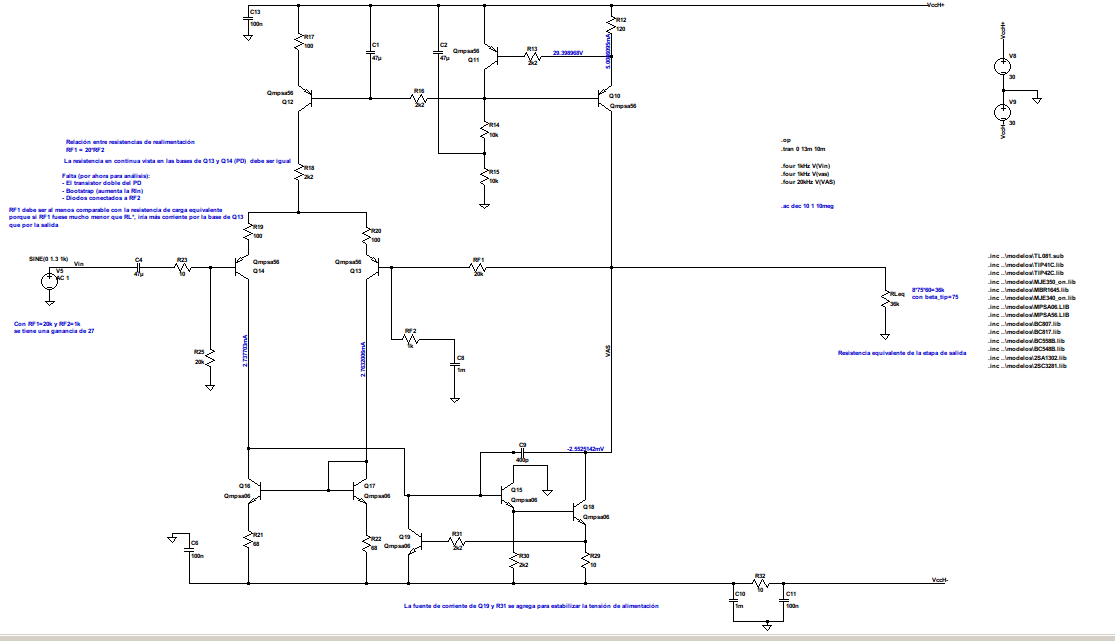
\includegraphics[scale=0.5]{sim_esq_vas.png}
	\caption{Primeras dos etapas.}
	\label{fig:sim_salida}
\end{figure}

\begin{figure}[H]
	\centering
	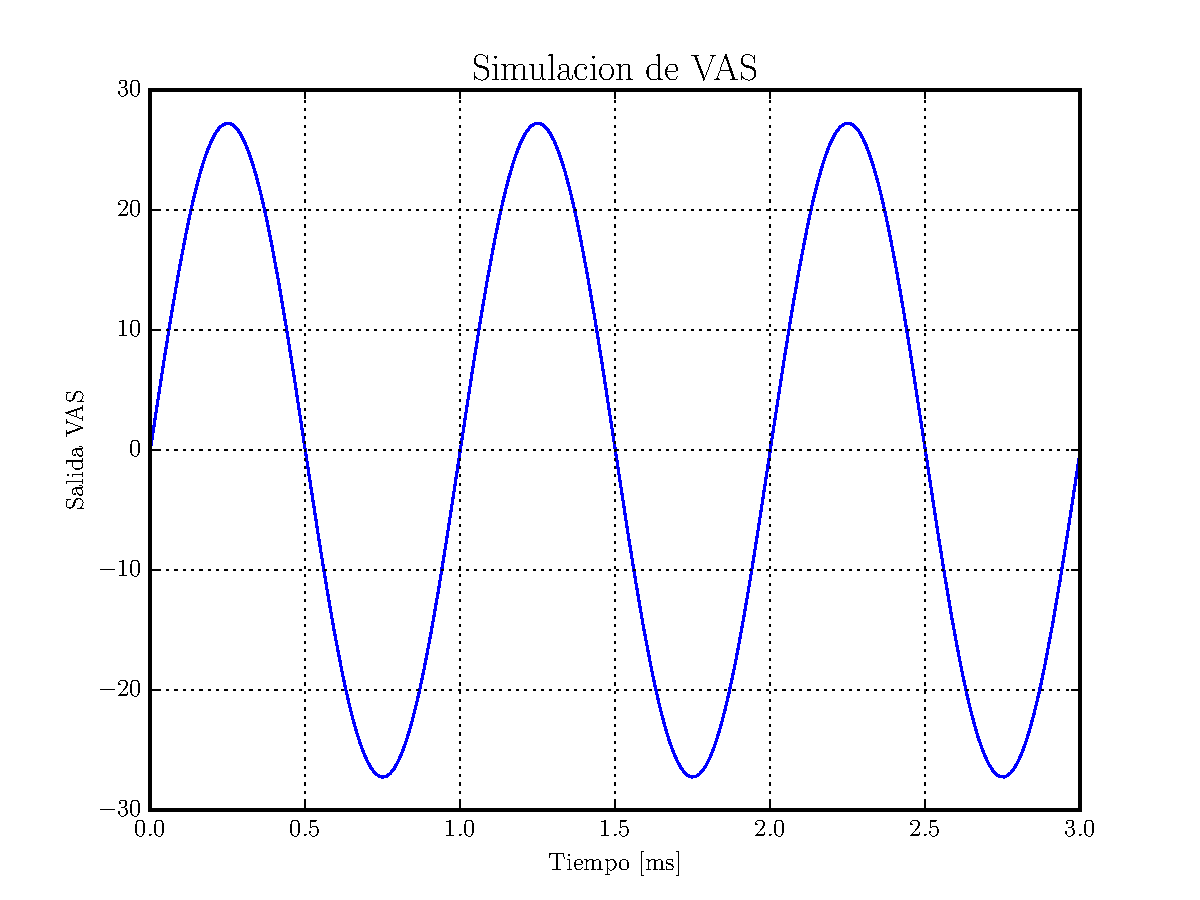
\includegraphics[scale=0.5]{sim_vas.pdf}
	\caption{Salida de la etapa VAS $\mathrm{THD}=0,000205\%$.}
	\label{fig:sim_vas}
\end{figure}

\begin{figure}[H]
	\centering
	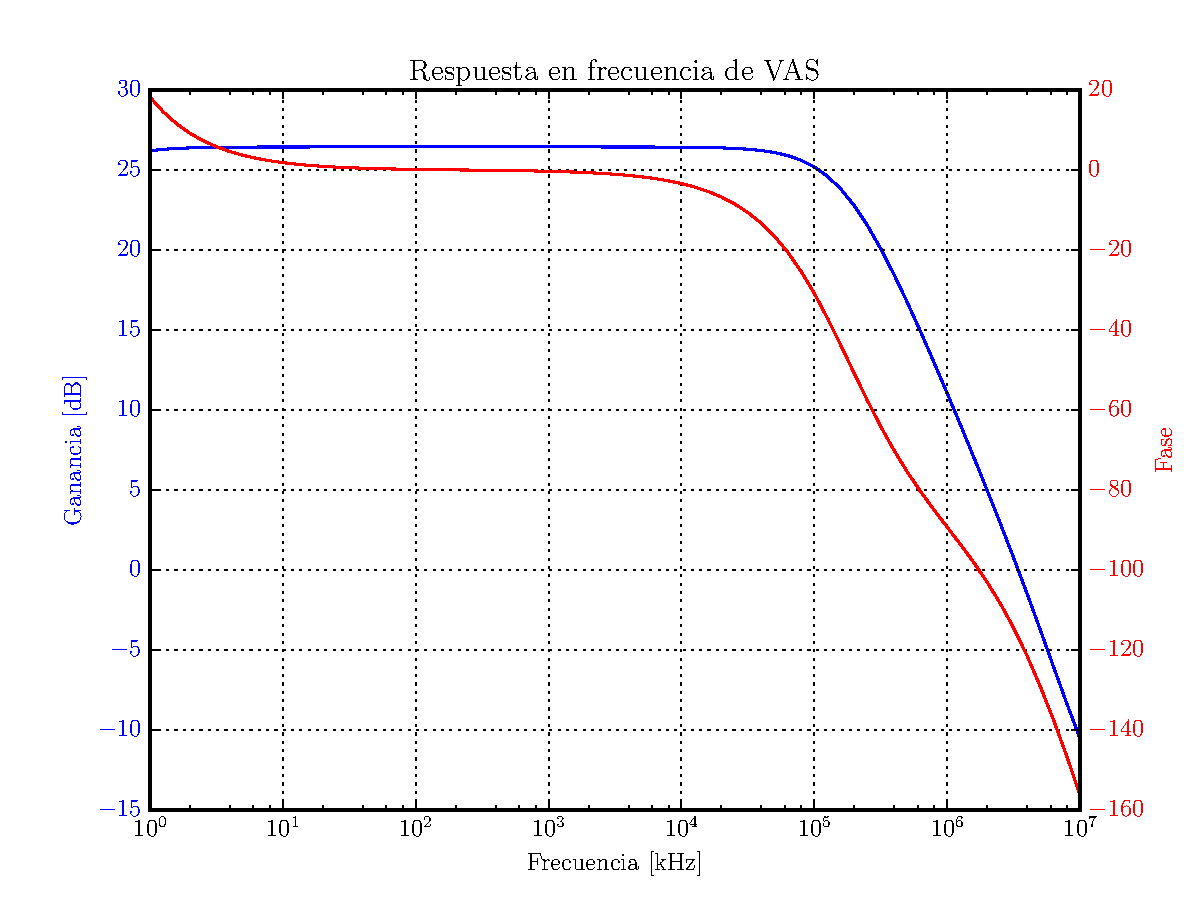
\includegraphics[scale=0.5]{sim_vas_bode.pdf}
	\caption{Respuesta en frecuencia de la etapa VAS.}
	\label{fig:sim_bode_vas}
\end{figure}

A partir de la figura \ref{fig:sim_bode_vas} se observa que el margen de fase resulta ser de $\SI{60}{\degree}$, se obtuvo ajustando el valor del capacitor de compensación $C2$ en $\SI{400}{\pico\farad}$.
